% !TEX root = saveliev_physics_general_course_2.tex
%!TEX TS-program = pdflatex
%!TEX encoding = UTF-8 Unicode


\chapter[ELECTROMAGNETIC WAVES]{ELECTROMAGNETIC WAVES}\label{chap:15}
\chaptermark{ELECTROMAGNETIC WAVES}

\section{The Wave Equation for
an Electromagnetic Field}\label{sec:15_1}

We established in Chapter \ref{chap:9} that a varying electric field sets up a magnetic one which, generally speaking, is also varying.
This varying magnetic field sets up an electric field, and so on.
Thus, if we use oscillating charges to produce a varying (alternating) electromagnetic field, then, in the space surrounding the charges a sequence of mutual transformations of an electric and a magnetic field propagating from point to point will appear.
This process will be periodic in both time and space and, consequently, will be a wave.

We shall show that the existence of electromagnetic waves follows from Maxwell's equations.
For a homogeneous, neutral ($\rho=0$), non-conducting ($\vec{j}=0$) medium with a constant permittivity $\varepsilon$ and a constant permeability $\mu$, we have
\begin{align*}
    \diffpartial{\vec{B}}{t} = \mu\mu_0\, \diffpartial{\vec{H}}{t},&\quad \diffpartial{\vec{D}}{t} = \varepsilon\varepsilon_0\, \diffpartial{\vec{E}}{t},\\
    \divop{\vec{B}} = \mu\mu_0 (\divop{\vec{H}}),&\quad \divop{\vec{D}} = \varepsilon\varepsilon_0 (\divop{\vec{E}}).
\end{align*}

\noindent
Consequently, Eqs. \eqref{eq:9_5}, \eqref{eq:7_3}, \eqref{eq:9_13}, and \eqref{eq:2_23} can be written as
follows:
\begin{align}
    \curlop{\vec{E}} &= - \mu\mu_0\, \diffpartial{\vec{H}}{t}, \label{eq:15_1}\\
    \divop{\vec{H}} &= 0, \label{eq:15_2}\\
    \curlop{\vec{H}} &= \varepsilon\varepsilon_0\, \diffpartial{\vec{E}}{t}, \label{eq:15_3}\\
    \divop{\vec{E}} &= 0. \label{eq:15_4}
\end{align}

Let us take a curl of both sides of \eqn{15_1}:
\begin{equation}\label{eq:15_5}
    \curlop{(\curlop{\vec{E}})} = - \mu\mu_0 \curlop{\parenthesis{\diffpartial{\vec{H}}{t}}}.
\end{equation}

\noindent
The symbol $\nabla$ denotes differentiation by coordinates.
A change in the sequence of differentiation with respect to the coordinates and time leads to the equation
\begin{equation*}
    \curlop{\parenthesis{\diffpartial{\vec{H}}{t}}} = \diffpartial{}{t}(\curlop{\vec{H}}).
\end{equation*}

\noindent
Making such a substitution in \eqn{15_5} and introducing the value given by \eqn{15_3} for the curl of $\vec{H}$ into the equation obtained, we have
\begin{equation}\label{eq:15_6}
    \curlop{(\curlop{\vec{E}})} = - \varepsilon\varepsilon_0 \mu\mu_0 \diffnpartial{\vec{E}}{t}{2}.
\end{equation}

According to \eqn{1_107}, $\curlop{(\curlop{\vec{E}})} = \gradop{(\divop{\vec{E}})} - \upDelta{\vec{E}}$.
Because of \eqn{15_4}, the first term of this expression is zero.
Consequently, the left-hand side of \eqn{15_6} is $-\upDelta{\vec{E}}$.
Thus, omitting the minus signs at both sides of the equation, we obtain
\begin{equation*}
    \upDelta{\vec{E}} = \varepsilon\varepsilon_0 \mu\mu_0\, \diffnpartial{\vec{E}}{t}{2}.
\end{equation*}

\noindent
According to \eqn{6_15}, we have $\varepsilon_0\mu_0=1/c$.
The equation can, therefore, be written in the form
\begin{equation}\label{eq:15_7}
    \upDelta{\vec{E}} = \frac{\varepsilon\mu}{c^2}\, \diffnpartial{\vec{E}}{t}{2}.
\end{equation}

\noindent
Expanding the Laplacian operator, we get
\begin{equation}\label{eq:15_8}
    \diffpartial{\vec{E}}{x}{2} + \diffpartial{\vec{E}}{y}{2} + \diffpartial{\vec{E}}{z}{2} = \frac{\varepsilon\mu}{c^2}\, \diffnpartial{\vec{E}}{t}{2}.
\end{equation}

Taking a curl of both sides of \eqn{15_3} and performing similar transformations, we arrive at the equation
\begin{equation}\label{eq:15_9}
    \diffpartial{\vec{H}}{x}{2} + \diffpartial{\vec{H}}{y}{2} + \diffpartial{\vec{H}}{z}{2} = \frac{\varepsilon\mu}{c^2}\, \diffnpartial{\vec{H}}{t}{2}.
\end{equation}

\noindent
Equations \eqref{eq:15_8} and \eqref{eq:15_9} are inseparably related to each other because they have been obtained from \eqns{15_1}{15_3} each
of which contains both $\vec{E}$ and $\vec{H}$.

Equations \eqref{eq:15_8} and \eqref{eq:15_9} are typical wave equations [see \eqn{14_24}].
Any function satisfying such an equation describes a wave.
The square root of the quantity that is the reciprocal of the coefficient of the time derivative gives the phase velocity of this wave.
Hence, \eqns{15_8}{15_9} point to the fact that electromagnetic fields can exist in the form of electromagnetic waves whose phase velocity is
\begin{equation}\label{eq:15_10}
    v = \frac{c}{\sqrt{\varepsilon\mu}}.
\end{equation}

\noindent
In a vacuum (\ie, when $\varepsilon=\mu=1$), the velocity of electromagnetic waves coincides with that of light in free space $c$.

\section{Plane Electromagnetic Wave}\label{sec:15_2}

Let us investigate a plane electromagnetic wave propagating in a neutral non-conducting medium with a constant permittivity $\varepsilon$ and
permeability $\mu$ ($\rho=0$, $\vec{j}=0$, $\varepsilon=\text{constant}$, $\mu=\text{constant}$).
We shall direct the $x$-axis at right angles to the wave surfaces.
Hence, $\vec{E}$ and $\vec{H}$, and, consequently, their components along the coordinate axes will not depend on the coordinates $y$ and $z$.
For this reason, Eqs. \eqref{eq:9_15}-\eqref{eq:9_18} can be simplified as follows:
\begin{align}
    & 0 = \mu\mu_0\, \diffpartial{H_x}{t},\quad  \diffpartial{E_z}{x} = \mu\mu_0\, \diffpartial{H_y}{t}, \quad \diffpartial{E_y}{x} = -\mu\mu_0\, \diffpartial{H_z}{t} \label{eq:15_11} \\
    & \diffpartial{B_x}{x} = \mu\mu_0\, \diffpartial{H_x}{x} = 0,\label{eq:15_12}
\end{align}

\begin{align}
    & 0 = \varepsilon\varepsilon_0\, \diffpartial{E_x}{t}, \quad  \diffpartial{H_z}{x} = -\varepsilon \varepsilon_0\, \diffpartial{E_y}{t}, \quad \diffpartial{H_y}{x} = \varepsilon\varepsilon_0\, \diffpartial{E_z}{t} \label{eq:15_13}\\
    & \diffpartial{D_x}{x} = \varepsilon \varepsilon_0\, \diffpartial{E_x}{x} = 0.\label{eq:15_14}
\end{align}

\noindent
Equation \eqref{eq:15_14} and the first of Eqs. \eqref{eq:15_13} show that $E_x$ can depend neither on $x$ nor on $t$.
Equation \eqref{eq:15_12} and the first of Eqs.
\eqref{eq:15_11} give the same result for $H_x$.
Hence, $E_x$ and $H_x$ differing from zero can be due only to constant homogeneous fields superposed onto the electromagnetic field of a wave.
The wave field itself cannot have components along the $x$-axis.
It thus follows that the vectors $\vec{E}$ and $\vec{H}$ are perpendicular to the direction of propagation of the wave, \ie, that electromagnetic waves are transverse.
We shall assume in the following that the constant fields are absent and that $E_x=H_x=0$.

The last two equations \eqref{eq:15_11} and the last two equations \eqref{eq:15_13} can be combined into two independent groups
\begin{align}
    \diffpartial{E_y}{x} &= -\mu\mu_0\, \diffpartial{H_z}{t},\quad \diffpartial{H_z}{x} = -\varepsilon\varepsilon_0\, \diffpartial{E_y}{t}, \label{eq:15_15} \\
    \diffpartial{E_z}{x} &= \mu\mu_0\, \diffpartial{H_y}{t},\quad \diffpartial{H_y}{x} = \varepsilon\varepsilon_0\, \diffpartial{E_z}{t}. \label{eq:15_16}
\end{align}

\noindent
The first group of equations relates the components $E_y$ and $H_z$, and the second group, the components $E_z$ and $H_y$.
Assume that there was initially set up a varying electric field $E_y$ directed along the $y$-axis.
According to the second of Eqs. \eqref{eq:15_15}, this field produces the magnetic field $H_z$ directed along the $z$-axis.
In accordance with the first of Eqs. \eqref{eq:15_15}, the field $H_z$ produces the electric field $E_y$, and so on.
Neither the field $E_z$ nor the field $H_y$ is produced.
Similarly, if the field $E_z$ was produced initially, then according to Eqs. \eqref{eq:15_16} the field $H_y$ will appear that will set up the field $E_z$, etc.
In this case, the fields $E_y$ and $H_z$ are not produced.
Thus, to describe a plane electromagnetic wave, it is sufficient to take one of the systems of equations \eqref{eq:15_15} or \eqref{eq:15_16} and to assume that the components in the other system equal zero.

Let us take Eqs. \eqref{eq:15_15} to describe a wave, assuming that $E_z=H_y=0$.
We shall differentiate the first equation with respect to $x$ and make the substitution $(\diffpartialin{}{x}) (\diffpartialin{H_z}{t}) = (\diffpartialin{}{t}) (\diffpartialin{H_z}{x})$.
Next introducing $\diffpartialin{H_z}{x}$ from the second equation, we get a wave equation for $E_y$:
\begin{equation}\label{eq:15_17}
    \diffnpartial{E_y}{x}{2} = \frac{\varepsilon\mu}{c^2}\, \diffnpartial{E_y}{t}{2}
\end{equation}

\noindent
(we have substituted $1/c^2$ for $\varepsilon_0 \mu_0$).
Differentiating the second of Eqs. \eqref{eq:15_15} with respect to $x$, we find a wave equation for $H_z$ after similar transformations:
\begin{equation}\label{eq:15_18}
    \diffnpartial{H_z}{x}{2} = \frac{\varepsilon\mu}{c^2}\, \diffnpartial{H_z}{t}{2}.
\end{equation}

\noindent
The equations obtained are a particular case of \eqns{15_8}{15_9}.

We remind our reader that $E_x=E_z=0$ and $H_x=H_y=0$, so that $E_y=E$ and $H_z=H$.
We have retained the subscripts $y$ and $z$ of $E$ and $H$ to stress the circumstance that the vectors $\vec{E}$ and $\vec{H}$ are directed along mutually perpendicular axes $y$ and $z$.

The simplest solution of \eqn{15_17} is the function
\begin{equation}\label{eq:15_19}
    E_y = \ab{E}{m} \cos(\omega t - kx + \alpha_1).
\end{equation}

\noindent
The solution of \eqn{15_18} is similar:
\begin{equation}\label{eq:15_20}
    H_z = \ab{H}{m} \cos(\omega t - kx + \alpha_2).
\end{equation}

\noindent
In these equations, $\omega$ is the frequency of the wave, $k$ is the wave number equal to $\omega/v$, and $\alpha_1$ and $\alpha_2$ are the initial phases of the oscillations at points with the coordinate $x=0$.

Introducing functions \eqref{eq:15_19} and \eqref{eq:15_20} into Eqs. \eqref{eq:15_15}, we get
\begin{align*}
    k\ab{E}{m} \sin(\omega t - kx + \alpha_1) &= \mu\mu_0 \omega \ab{H}{m} \sin(\omega t - kx + \alpha_2),\\
    k\ab{H}{m} \sin(\omega t - kx + \alpha_2) &= \varepsilon\varepsilon_0 \omega \ab{E}{m} \sin(\omega t - kx + \alpha_1).
\end{align*}

\noindent
For these equations to be satisfied, equality of the initial phases $\alpha_1$ and $\alpha_2$ is needed.
In addition, the following relations must be observed
\begin{align*}
    k\ab{E}{m} &= \mu\mu_0 \omega \ab{H}{m},\\
    k\ab{H}{m} &= \varepsilon\varepsilon_0 \omega \ab{E}{m}.
\end{align*}

\noindent
Multiplying these two equations, we find that
\begin{equation}\label{eq:15_21}
    \varepsilon\varepsilon_0 \ab{E}{m}^2 = \mu\mu_0 \ab{H}{m}^2.
\end{equation}

\noindent
Thus, the oscillations of the electric and magnetic vectors in an electromagnetic wave occur with the same phase ($\alpha_1=\alpha_2$), while the amplitudes of these vectors are related by the expression
\begin{equation}\label{eq:15_22}
    \ab{E}{m} \sqrt{\varepsilon\varepsilon_0} = \ab{H}{m} \sqrt{\mu\mu_0}.
\end{equation}

\noindent
For a wave propagating in a vacuum, we have
\begin{equation}\label{eq:15_23}
    \frac{\ab{E}{m}}{\ab{H}{m}} = \parenthesis{\frac{\mu_0}{\varepsilon_0}}^{1/2} = \sqrt{4\pi \times \num{e-7} \times 4\pi \times \num{9e9}} = 120\pi \approx 377.
\end{equation}

\noindent
In the Gaussian system of units, \eqn{15_22} becomes
\begin{equation}\label{eq:15_24}
    \ab{E}{m} \sqrt{\varepsilon} = \ab{H}{m} \sqrt{\mu}.
\end{equation}

Consequently, for a vacuum, we have $\ab{E}{m}=\ab{H}{m}$ ($\ab{E}{m}$ is measured in cgse units, and $\ab{H}{m}$ in cgsm ones).

Multiplying \eqn{15_19} by the unit vector $\vecuni{y}$ of the $y$-axis ($E_y\vecuni{y}=\vec{E}$), and \eqn{15_20} by the unit vector $\vecuni{z}$ of the $z$-axis ($H_z\vecuni{z}=\vec{H}$), we get equations for a plane electromagnetic wave in the vector form
\begin{equation}\label{eq:15_25}
    \begin{split}
        \vec{E} &= \ab{\vec{E}}{m} \cos(\omega t - kx)\\
        \vec{H} &= \ab{\vec{H}}{m} \cos(\omega t - kx)
    \end{split}
\end{equation}

\noindent
(we have assumed that $\alpha_1=\alpha_2=0$).

Figure \ref{fig:15_1} shows an ``instantaneous photograph'' of a plane electromagnetic wave.
A glance at the figure shows that the vectors $\vec{E}$ and $\vec{H}$ form a right-handed system with the direction of propagation of the wave.
At a fixed point of space, the vectors $\vec{E}$ and $\vec{H}$ vary with time according to a harmonic law.
They simultaneously grow from zero, and next reach their maximum value in one-fourth of a period; if $\vec{E}$ is directed upward, then, $\vec{H}$ is directed to the right (we look along the direction of propagation of the wave).
In another one-fourth of a period, both vectors simultaneously vanish.
Next, they again reach their maximum value, but this time, $\vec{E}$ is directed downward, and $\vec{H}$ to the left.
And, finally, upon completion of a period of oscillation, the vectors again vanish.
Such changes in the vectors $\vec{E}$ and $\vec{H}$ occur at all points of space, but with a shift in phase determined by the distance between the points measured along the $x$-axis.

\begin{figure}[t]
	\begin{center}
		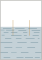
\includegraphics[scale=1]{figures/ch_15/fig_15_1.pdf}
		\caption[]{}
		\label{fig:15_1}
	\end{center}
	\vspace{-0.8cm}
\end{figure}

\section{Experimental Investigation of Electromagnetic Waves}\label{sec:15_3}

The first experiments with non-optical electromagnetic waves were conducted in 1888 by the German physicist Heinrich Hertz (1857-1894).
Hertz produced waves with the aid of a vibrator which he had invented.
The vibrator consisted of two rods separated by a spark gap.
When a high voltage was fed to the vibrator from an induction coil, a spark jumped through the gap.
It shorted the latter, and damped electrical oscillations were set up in the vibrator (\fig{15_2}; the chokes shown in the figure were intended to prevent the high-frequency current from branching off into the inductor winding).
During the time the spark burned, a great number of oscillations were completed.
They produced a train of electromagnetic waves whose length was approximately twice that of the vibrator.
By placing vibrators of various length at the focus of a concave parabolic mirror, Hertz obtained directed plane waves whose length ranged from \SIrange{0.6}{10}{\metre}.

\begin{figure}[t]
	\begin{center}
		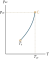
\includegraphics[scale=1]{figures/ch_15/fig_15_2.pdf}
		\caption[]{}
		\label{fig:15_2}
	\end{center}
	\vspace{-0.8cm}
\end{figure}

Hertz also studied the emitted wave with the aid of a half-wave vibrator having a small spark gap at its middle.
When such a vibrator was placed parallel to the electric field strength vector of the wave, oscillations of the current and voltage were produced in it.
Since the length of the vibrator was equal to $\lambda/2$, the oscillations in it owing to resonance reached such an intensity that they caused small sparks to jump across the spark gap.

Hertz reflected and refracted electromagnetic waves with the aid of large metal mirrors and an asphalt prism (over \SI{1}{\metre} in size and with a mass of \SI{1200}{\kilo\gram}).
He discovered that both these phenomena obey the laws established in optics for light waves.
By reflecting a running plane wave with the aid of a metal mirror to the opposite direction, Hertz obtained a standing wave.
The distance between the nodes and antinodes of the wave made it possible to find its length $\lambda$.
By multiplying $\lambda$ by the frequency of oscillations $\nu$ of the vibrator, the velocity of the electromagnetic waves was determined, and it was found to be close to $c$.
By placing a grate of parallel copper wires in the path of waves, Hertz discovered that the intensity of the waves passing through the grate changes very greatly when the grate is rotated about the beam. When the wires forming the grate were perpendicular to the vector $\vec{E}$, the wave passed through the grate without any hindrance.
When the wires were arranged parallel to $\vec{E}$, the wave did not pass through the grate.
Thus, the transverse nature of electromagnetic waves was proved.

Hertz's experiments were continued by the Russian physicist Pyotr Lebedev (1866-1912), who in 1894 obtained electromagnetic waves \SI{6}{\milli\metre} long and studied how they travel in crystals.
He detected double refraction of the waves (see \sect{19_3}).

In 1896, the Russian inventor Aleksandr Popov (1859-1905) for the first time in history transmitted a message over a distance of about \SI{250}{\metre} with the aid of electromagnetic waves (the words ``Heinrich Hertz'' were transmitted).
This laid the foundation of radio engineering.

\section{Energy of Electromagnetic Waves}\label{sec:15_4}

Electromagnetic waves transfer energy.
According to \eqn{14_46}, the density of the energy flux can be obtained by multiplying the energy density by the wave velocity.

The density of the energy of an electromagnetic field $w$ consists of the density of the energy of the electric field [determined by \eqn{4_10}] and that of the energy of the magnetic field [determined
by \eqn{8_40}]:
\begin{equation}\label{eq:15_26}
    w = w_E + w_H = \frac{\varepsilon\varepsilon_0 E^2}{2} + \frac{\mu\mu_0 H^2}{2}.
\end{equation}

\noindent
The vectors $\vec{E}$ and $\vec{H}$ at a given point of space vary in the same phase\footnote{This holds only for a non-conducting medium. The phases of $\vec{E}$ and $\vec{B}$ do not coincide in a conducting medium.}.
Therefore, \eqn{15_22} giving the relation between the amplitude values of $E$ and $H$ also holds for their instantaneous values.
It thus follows that the densities of the energy of the electric and magnetic fields of a wave are identical at each moment of time: $w_E = w_H$.
We can, therefore, write that
\begin{equation}\label{eq:15_27}
    w = 2 w_E = \varepsilon\varepsilon_0 E^2.
\end{equation}

Taking advantage of the fact that $E\sqrt{\varepsilon\varepsilon_0} = H \sqrt{\mu\mu_0}$, we can write \eqn{15_27} in the form
\begin{equation*}
    w = \sqrt{\varepsilon\varepsilon_0\mu\mu_0} EH = \frac{1}{v} EH,
\end{equation*}

\noindent
where $v$ is the velocity of an electromagnetic wave [see \eqn{15_10}].

Multiplying the expression found for $w$ by the wave velocity $v$, we get the magnitude of the energy flux density vector
\begin{equation}\label{eq:15_28}
    S = w v = EH.
\end{equation}

\noindent
The vectors $\vec{E}$ and $\vec{H}$ are mutually perpendicular and form a right-handed system with the direction of propagation of the wave.
For this reason, the direction of the vector $\vecprod{E}{H}$ coincides with that of energy transfer, and the magnitude of this vector is $EH$.
Hence, the vector of the density of the electromagnetic energy flux can be written as the vector product of $\vec{E}$ and $\vec{H}$:
\begin{equation}\label{eq:15_29}
    \vec{S} = \vecprod{E}{H}.
\end{equation}

\noindent
The vector $\vec{S}$ is known as the \textbf{Poynting vector}.

By analogy with \eqn{14_50}, the flux $\Phi$ of electromagnetic energy through surface $\ab{A}{s}$ can be found by integration:
\begin{equation}\label{eq:15_30}
    \Phi = \oint_{\ab{A}{s}} \vec{S} \ccdot \ab{\derivec{A}}{s}
\end{equation}

\noindent
[in \eqn{14_50} the surface area was designated by the symbol $S$; since this symbol is used to designate the Poynting vector, we were forced to introduce the symbol $\ab{A}{s}$ for the surface
area].

Let us consider a portion of a homogeneous cylindrical conductor through which a steady current is flowing (\fig{15_3}) as an example of applying \eqns{15_29}{15_30}.
We shall first consider that extraneous forces are absent on this portion of the conductor.
Hence, according to \eqn{5_22}, the following relation is observed at each point of the conductor:
\begin{equation*}
    \vec{j} = \sigma \vec{E} = \frac{1}{\rho} \vec{E}.
\end{equation*}

\begin{figure}[t]
	\begin{center}
		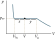
\includegraphics[scale=1]{figures/ch_15/fig_15_3.pdf}
		\caption[]{}
		\label{fig:15_3}
	\end{center}
	\vspace{-0.8cm}
\end{figure}

The steady current is distributed over the cross section of the conductor with an identical density $\vec{j}$.
Hence, the electric field within the limits of the portion of the conductor shown in \fig{15_3} will
be homogeneous.
Let us mentally separate a cylindrical volume of radius $r$ and length $l$ inside the conductor.
At each point on the side surface of this cylinder, the vector $\vec{H}$ is perpendicular to the vector $\vec{E}$ and is directed tangentially to the surface.
The magnitude of $\vec{H}$ is $jr/2$ [according to \eqn{7_10}, we have $2\pi rH = j\pi r^2$].
Thus, the Poynting vector given by \eqn{15_29} is directed toward the axis of the conductor at each point on the surface and has the magnitude $S=EH=Ej r^2/2$.
Multiplying $S$ by the side surface area of the cylinder $\ab{A}{s}$ equal to $2\pi rl$, we find that the following flux of electromagnetic energy enters the volume we are considering:
\begin{equation}\label{eq:15_31}
    \Phi = S \ab{A}{s} = \frac{1}{2} Ejr \times 2\pi rl = Ej \times \pi r^2 l = Ej \times V,
\end{equation}

\noindent
where $V$ is the volume of the cylinder.

According to \eqn{6_4}, $Ej = pj^2$ is the amount of heat liberated in unit time per unit volume of the conductor.
Consequently, \eqn{15_31} indicates that the energy liberated in the form of Lenz-Joule heat is supplied to the conductor through its side surface in the form of energy of an electromagnetic field.
The energy flux gradually weakens with deeper penetration into the conductor (both the Poynting vector and the surface through which the flux passes diminish) as a result of absorption of energy and its conversion into heat.

Now, let us assume that extraneous forces whose field is homogeneous are exerted within the limits of the portion of the conductor we are considering ($\vec{E}^*=\text{constant}$).
In this case according to \eqn{5_25}, at each point of the conductor we have
\begin{equation*}
    \vec{j} = \sigma \parenthesis{\vec{E} + \vec{E}^*} = \frac{1}{\rho} \parenthesis{\vec{E} + \vec{E}^*},
\end{equation*}

\noindent
whence
\begin{equation}\label{eq:15_32}
    \vec{E} = \rho \vec{j} - \vec{E}^*.
\end{equation}

\noindent
We shall consider that the extraneous forces on the portion of the circuit being considered do not hamper the flow of the current, but facilitate it.
This signifies that the direction of $\vec{E}^*$ coincides with that of $\vec{j}$.
Let us assume that the relation $\rho j = E^*$ is observed.
Hence, according to \eqn{15_32}, the electrostatic field strength $\vec{E}$ at each point vanishes, and there is no flux of electromagnetic energy through the side surface.
In this case, heat is liberated at the expense of the work of the extraneous forces.

If the relation $E^*>\rho j$ holds, then, as can be seen from \eqn{15_32}, the vector $\vec{E}$ will be directed oppositely to the vector $\vec{j}$.
In this case, the vectors $\vec{E}$ and $\vec{S}$ will have directions opposite to those shown in \fig{15_3}.
Hence, instead of flowing in, electromagnetic energy
flows out through the side surface of the conductor into the space surrounding it.

In summarizing, we can say that in the closed circuit of a steady current, the energy from the sections where extraneous forces act is transmitted to other sections of the circuit not along the conductors, but through the space surrounding the conductors in the form of a flux of electromagnetic energy characterized by the vector $\vec{S}$.

\section{Momentum of Electromagnetic Field}\label{sec:15_5}

An electromagnetic wave absorbed in a body imparts a momentum to the body, \ie, exerts a pressure on it.
This can be shown by the following example.
Assume that a plane wave impinges normally onto a flat surface of a weakly conducting body with $\varepsilon$ and $\mu$ equal to unity (\fig{15_4}).
The electric field of the wave produces a current of density $\vec{j} = \sigma\vec{E}$ in the body.
The magnetic field of the wave will act on the current with a force whose value per unit volume of the body can be found by \eqn{6_43}:
\begin{equation*}
    \ab{\vec{F}}{u.v} = \vecprod{j}{B} = \mu_0 (\vecprod{k}{H}).
\end{equation*}

\noindent
The direction of this force, as can be seen from \fig{15_4}, coincides with the direction of propagation of the wave.

\begin{figure}[t]
	\begin{center}
		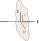
\includegraphics[scale=1]{figures/ch_15/fig_15_4.pdf}
		\caption[]{}
		\label{fig:15_4}
	\end{center}
	\vspace{-0.8cm}
\end{figure}

The momentum
\begin{equation}\label{eq:15_33}
    \deriv{K} = \ab{F}{u.v}\, \deriv{l} = \mu_0 j H\, \deriv{l}
\end{equation}

\noindent
is imparted to a surface layer having a unit area and a thickness of $\deriv{l}$ in unit time (the vectors $\vec{j}$ and $\vec{H}$ are mutually perpendicular).
The energy absorbed in this layer in unit time is
\begin{equation}\label{eq:15_34}
    \deriv{W} = jE\, \deriv{l}.
\end{equation}

\noindent
It is liberated in the form of heat.

The momentum given by \eqn{15_33} and the energy [\eqn{15_34}] are imparted to the layer by the wave.
Let us take their ratio, omitting the differential symbols as superfluous:
\begin{equation*}
    \frac{K}{W} = \mu_0 \frac{H}{E}.
\end{equation*}

\noindent
Taking into account that $\mu_0 H^2=\varepsilon_0 E^2$, we get
\begin{equation*}
    \frac{K}{W} = \sqrt{\varepsilon_0\mu_0} = \frac{1}{c}.
\end{equation*}

\noindent
It thus follows that an electromagnetic wave carrying the energy $W$ has the momentum
\begin{equation}\label{eq:15_35}
    K = \frac{1}{c} W.
\end{equation}

\noindent
The same relation between the energy and the momentum holds for particles with a zero rest mass [see Eq. (8.57) of Vol. I].
This is not surprising because according to quantum notions, an electromagnetic wave is equivalent to a flux of photons, \ie, particles whose mass (we have in mind their rest mass) is zero.

Examination of \eqn{15_35} shows that the density of the momentum (\ie, the momentum of unit volume) of an electromagnetic field is
\begin{equation}\label{eq:15_36}
    \ab{K}{u.v} = \frac{1}{c} w.
\end{equation}

\noindent
The energy density is related to the magnitude of the Poynting vector by the expression $S = wc$. Substituting $S/c$ for $w$ in \eqn{15_36} and taking into account that the directions of the vectors $\vec{K}$ and $\vec{S}$ coincide, we can write that
\begin{equation}\label{eq:15_37}
    \ab{\vec{K}}{u.v} = \frac{1}{c^2} \vec{S} = \frac{1}{c^2} (\vecprod{E}{H}).
\end{equation}

We shall note that when energy of any kind is transferred, the density of the energy flux equals the density of the momentum multiplied by $c^2$.
Let us consider, for example, a collection of particles distributed in space with the density $n$ and flying with a velocity $v$ identical in magnitude and direction.
In this case, the density of the momentum
\begin{equation}\label{eq:15_38}
    \ab{\vec{K}}{u.v} = n \frac{m\vec{v}}{\sqrt{1 - \parenthesis{v^2/c^2}}}.
\end{equation}

\noindent
The particles carry along energy whose density flux $\vec{j}_W$ equals the density of the particle flux multiplied by the energy of one particle:
\begin{equation}\label{eq:15_39}
    \vec{j}_W = n \vec{v} \frac{mc^2}{\sqrt{1 - \parenthesis{v^2/c^2}}}.
\end{equation}

\noindent
It follows from \eqns{15_38}{15_39} that
\begin{equation}\label{eq:15_40}
    \ab{\vec{K}}{u.v} = \frac{1}{c^2} \vec{j}_W.
\end{equation}

Assume that an electromagnetic wave falling normally on a body is completely absorbed by the body.
Hence, a unit of surface area of the body receives in unit time the momentum of the wave enclosed in a cylinder with a base area of unity and an altitude of $c$.
According to \eqn{15_36}, this momentum is $(w/c)c=w$.
At the same time, the momentum imparted to a unit surface area in unit time equals the pressure $p$ on the surface.
Hence, for an absorbing surface, we have $p = w$.
This quantity pulsates with a very high frequency.
We can, therefore, measure its time-averaged value in practice. Thus,
\begin{equation}\label{eq:15_41}
    p = \average{w}.
\end{equation}

\noindent
For an ideally reflecting surface, the pressure will be double this value.

The value of the pressure calculated by \eqn{15_41} is very small.
For example, at a distance of \SI{1}{\metre} from a source of light having an intensity of a million candelas, the pressure is only about \SI{e-7}{\pascal} (about \SI{e-9}{\gf\per\centi\metre\squared}).
Pyotr Lebedev succeeded in measuring the pressure of light.
By carrying out experiments requiring great inventiveness and skill, Lebedev measured the pressure of light on solids in 1900, and on gases in 1910.
The results of the measurements completely agreed with Maxwell's theory.

\section{Dipole Emission}\label{sec:15_6}

An oscillating electric dipole is the simplest system emitting electromagnetic waves.
An example of such a dipole is the system formed by a fixed point charge $+q$ and a point charge $-q$ oscillating near it (\fig{15_5}).
The dipole electric moment of this system varies in time according to the law
\begin{equation}\label{eq:15_42}
    \vec{p} = -q \vec{r} = - ql \hatvec{e} \cos(\omega t) = \ab{\vec{p}}{m} \cos(\omega t),
\end{equation}

\noindent
where $\vec{r}$ is the position vector of the charge $-q$, $l$ the amplitude of oscillations, $\hatvec{e}$ is the unit vector directed along the dipole axis, and $\ab{\vec{p}}{m} =-gl\hatvec{e}$.

\begin{figure}[t]
	\begin{minipage}[t]{0.48\linewidth}
		\begin{center}
			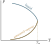
\includegraphics[scale=1]{figures/ch_15/fig_15_5.pdf}
			\caption[]{}
			\label{fig:15_5}
		\end{center}
	\end{minipage}
	\hfill{ }%space{-0.05cm}
	\begin{minipage}[t]{0.48\linewidth}
		\begin{center}
			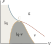
\includegraphics[scale=1]{figures/ch_15/fig_15_6.pdf}
			\caption[]{}
			\label{fig:15_6}
		\end{center}
	\end{minipage}
\vspace{-0.4cm}
\end{figure}

Acquaintance with such an emitting system is especially important in connection with the fact that many questions of the interaction of radiation with a substance can be explained classically proceeding from the notion of atoms as of systems of charges containing electrons that are capable of performing harmonic oscillations about their equilibrium position.

Let us consider the radiation of a dipole whose dimensions are small in comparison with the wavelength ($l\ll\lambda$).
Such a dipole is called \textbf{elementary}.
The pattern of the electromagnetic field in direct proximity to the dipole is very complicated.
It becomes simplified quite greatly in the so-called \textbf{wave zone} of the dipole that begins at distances $r$ considerably exceeding the wavelength ($r\gg\lambda$).
If a wave is propagating in a homogeneous isotropic medium, then its wavefront in the wave zone will be spherical (\fig{15_6}).
The vectors $\vec{E}$ and $\vec{H}$ at each point are mutually perpendicular and are perpendicular to the ray, \ie, to the position vector drawn to the given point from the centre of the dipole.

Let us call sections of the wavefront by planes passing through the dipole axis \textbf{meridians}, and by planes perpendicular to the dipole axis \textbf{parallels}.
We can now say that the vector $\vec{E}$ at each point of a wave zone is directed along a tangent to the meridian, and the vector $\vec{H}$ along a tangent to the parallel.
If we look along the ray $r$, then the instantaneous pattern of the wave will be the same as shown in \fig{15_5}, the only difference being that the amplitude in motion along the ray gradually diminishes.

At each point, the vectors $\vec{E}$ and $\vec{H}$ oscillate according to the law $\cos(\omega t - kr)$.
The amplitudes $\ab{\vec{E}}{m}$ and $\ab{\vec{H}}{m}$ depend on the distance $r$ to the emitter and on the angle a between the direction of the position vector $\vec{r}$ and the dipole axis (see \fig{15_6}).
This dependence has the following form for a vacuum:
\begin{equation*}
    \ab{E}{m} \propto \ab{H}{m} \propto \frac{1}{r} \sin\theta.
\end{equation*}

\noindent
The average value of the density of the energy flux $\average{S}$ is proportional to the product $\ab{E}{m}\ab{H}{m}$, consequently,
\begin{equation}\label{eq:15_43}
    \average{S} \propto \frac{1}{r^2} \sin^2\theta.
\end{equation}

\noindent
A glance at this expression shows that the wave intensity changes along the ray (at $\theta = \text{constant}$) in inverse proportion to the square of the distance from the emitter.
In addition, it depends on the angle $\theta$.
The emission of a dipole is the greatest in directions at right angles to its axis ($\theta = \pi/2$).
There is no emission in the directions coinciding with the axis ($\theta = 0$ and $\pi$).
How the intensity depends on the angle $\theta$ is shown very illustratively with the aid of a \textbf{dipole directional diagram} (\fig{15_7}).
This diagram is constructed so that the length of the segment it intercepts on a ray conducted from the
centre of the dipole gives the intensity of emission at the angle $\theta$.

The corresponding calculations show that the \textbf{radiant power} $P$ of a dipole (\ie, the energy emitted in all directions in unit time) is
proportional to the square of the second time derivative of the dipole moment:
\begin{equation}\label{eq:15_44}
    P \propto \ddot{\vec{p}}^2.
\end{equation}

\begin{figure}[t]
	\begin{center}
		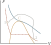
\includegraphics[scale=1]{figures/ch_15/fig_15_7.pdf}
		\caption[]{}
		\label{fig:15_7}
	\end{center}
	\vspace{-0.8cm}
\end{figure}

\noindent
According to \eqn{15_42}, $\ddot{\vec{p}}^2=\ab{p}{m}^2\omega^4\cos^2(\omega t)$.
Introduction of this value into expression \eqref{eq:15_44} yields
\begin{equation}\label{eq:15_45}
    P \propto \ab{p}{m}^2 \omega^4 \cos(\omega t).
\end{equation}

\noindent
Time averaging of this expression gives
\begin{equation}\label{eq:15_46}
    \average{P} \propto \ab{p}{m}^2 \omega^4.
\end{equation}

\noindent
Thus, the average radiant power of a dipole is proportional to the square of the amplitude of the electric dipole moment and to the fourth power of the frequency.
Therefore, at a low frequency, the emission of electrical systems (for instance, industrial frequency alternating current transmission lines) is insignificant.

According to \eqn{15_42}, we have $\ddot{\vec{p}}=-q\ddot{\vec{r}}=-q\vec{a}$, where $\vec{a}$ is the acceleration of an oscillating charge.
Substitution of this expression for $\ddot{\vec{p}}$ in \eqn{15_44} yields\footnote{The constant of proportionality when SI units are used is $\sqrt{\mu_0/\varepsilon_0}/(6\pi c^2)$, and when units of the Gaussian system are used is $2/(3c^3)$.}:
\begin{equation}\label{eq:15_47}
    P \propto q^2 \vec{a}^2.
\end{equation}

\noindent
Expression \eqref{eq:15_47} determines the radiant power not only for oscillations, but also for arbitrary motion of a charge.
A charge travelling with acceleration produces electromagnetic waves, and the radiated power is proportional to the square of the charge and the
square of the acceleration.
For example, the electrons accelerated in a betatron (see \sect{10_5}) lose energy as a result of radiation mainly due to centripetal acceleration $\ab{a}{n}=v^2/r$.
According to expression \eqref{eq:15_47}, the amount of energy lost grows greatly with an increasing velocity of the electrons in the betatron (in proportion to $v^4$).
Hence, the possible acceleration of electrons in a betatron is limited to about \SI{500}{\mega\electronvolt} (at a velocity corresponding to this value, the losses due to radiation become equal to the energy imparted to the electrons by the vortex electric field).

A charge performing harmonic oscillations emits a monochromatic wave with a frequency equal to that of the charge oscillations.
If the acceleration $\vec{a}$ of the charge does not change according to a harmonic law, then the radiation consists of a set of waves of different
frequencies.

According to expression \eqref{eq:15_47}, the intensity vanishes when $\vec{a}=0$.
Consequently, \textit{an electron travelling with a constant velocity does not emit electromagnetic waves}.
This holds, however, only for the case when the velocity of an electron $\ab{v}{el}$ does not exceed the speed of light $\ab{v}{l}=c/\sqrt{\varepsilon\mu}$ in the medium in which the electron is travelling.
When $\ab{v}{el}>\ab{v}{l}$, radiation is observed.
It was discovered in 1934 by the Soviet physicists Sergei Vavilov (1891-1951) and Pavel Cerenkov (born 1904).

% \begin{table}[!b]
% 	\renewcommand{\arraystretch}{1.2}
% 	\caption{}
% 	\vspace{-0.6cm}
% 	\label{table:14_1}
% 	\begin{center}\resizebox{0.65\linewidth}{!}{
% 			\begin{tabular}{lc}
% 				\toprule[1pt]
% 				\textbf{Sound} & \textbf{Loudness level}, \si{\decibel}\\
% 				\midrule[0.5pt]\midrule[0.5pt]
% 				\\
% 				\bottomrule[1pt]
% 			\end{tabular}
% 	}\end{center}
% \end{table}
